\section{Problema de planificación de producción tipo taller (JSP)}

Dentro de los problemas de planificación, el JSP modela un taller en el que hay $m$ máquinas, cada una de las cuales puede hacer varios tipos 
de procedimientos pero solo puede hacer uno de ellos a la vez. 
%
Se requiere completar $n$ trabajos, cada uno de los cuales está compuesto por $m$ operaciones, una por cada máquina en el taller, y que deben 
procesarse en un orden específico y por un tiempo específico en cada una de ellas. De este modo una operación solo puede comenzar a procesarse cuando su operación precedente en el trabajo y su operación precedente en la máquina ya han sido procesadas. Es decir que cada operación tiene dos tipos de dependencias, las propias de su trabajo y las de la máquina en donde ha de ser procesada.

Por ejemplo una panadería puede modelarse del siguiente modo; las herramientas como batidora, rodillo, horno, etc. pueden representarse como las
$m$ máquinas que se utilizan en un orden determinado para hacer $n$ distintos tipos de pan, los cuales pueden representarse como los trabajos 
a completar.

Las secuencias y tiempos de procesamiento para cada trabajo deben de especificarse para definir el problema. 
%
Habitualmente se presentan en una tabla de $n$ renglones por $m$ columnas esto se conoce como una instancia del JSP. 
%
Para cada renglón, las columnas contienen, de forma ordenada, la máquina en que debe procesarse el trabajo en cada paso y el tiempo 
que toma procesarlo. 
%
Por ejemplo en la tabla~\ref{tab:inst} se presenta una instancia del JSP con 3 máquinas y 2 trabajos. 
%
En esta instancia el trabajo 1 debe procesarse primero en la máquina 0 por 75 unidades de tiempo, luego en la máquina 2 por 54 unidades de tiempo y 
por último en la máquina 1 por 59 unidades de tiempo.

El problema a resolver consiste en hallar una planificación que sea óptima en algún sentido y respete los requisitos impuestos (orden y no concurrencia de diversas
operaciones).
%
Así, una planificación consiste en asignar tiempos de inicio y fin a cada operación respetando el orden requerido para cada trabajo. 

\subsection{Tipos de planificaciones}
Independientemente de cómo se representen o como se construyan, las planificaciones pueden clasificarse en varios conjuntos. Dentro del conjunto de planificaciones factibles se pueden distinguir tres subconjuntos de interés para el presente trabajo~\cite{sprecher1995semi}:
\begin{itemize}
    \item \textbf{Planificaciones semi-activas} Son aquellas en las que el tiempo de inicio de cada operación no puede disminuirse sin modificar el orden especificado en la planificación. De modo más intuitivo son aquellas en las que una máquina solo deja de trabajar porque la dependencia de la operación a procesar no ha sido procesada o porque ya terminó todo lo que tenía asignado.
    \item \textbf{Planificaciones activas} Son a su vez un subconjunto de las planificaciones activas y se definen como las planificaciones en las que no es posible disminuir el tiempo de inicio de ninguna operación sin aumentar el tiempo de inicio de otra. 
    \item \textbf{Planificaciones óptimas} Es el conjunto conformado por las planificaciones con el menor makespan posible. Este conjunto contiene planificaciones activas~\cite{Ponsich2013} aunque puede o no contener otras planificaciones que solo son factibles.
\end{itemize}

La relación entre estos conjuntos se ilustra en la figura \ref{fig:solspace}. 


\begin{figure}[H]
    \centering
    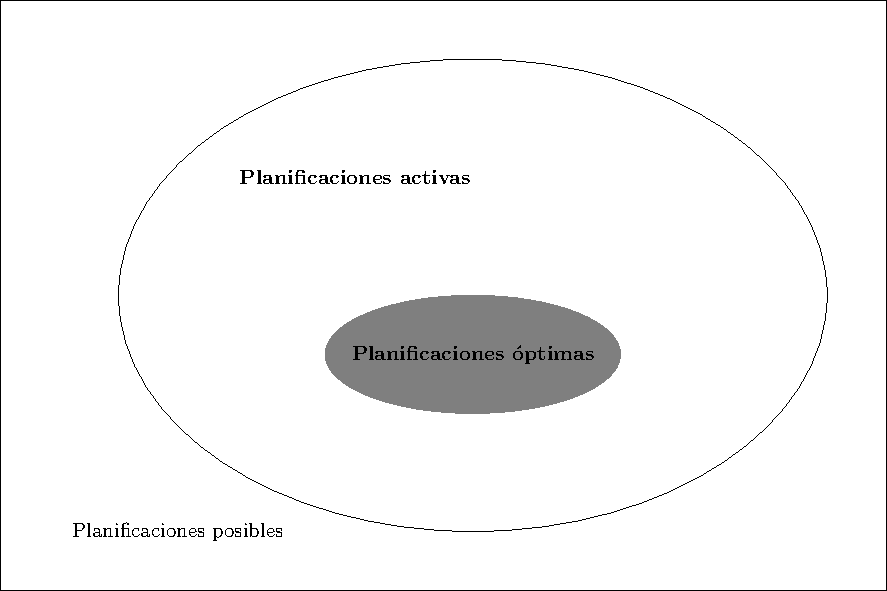
\includegraphics[scale=.8]{Imagenes/solspace.pdf}
    \caption{Subconjuntos de planificaciones. El área sombreada puede ser una intersección vacía}
    \label{fig:solspace}
\end{figure}

Es importante mencionar que el conjunto de las planificaciones factibles puede ser de tamaño arbitrario porque para cualquier planificación factible podemos insertar intervalos de tiempo inactivo de duración arbitraria entre operaciones en cualquier máquina sin alterar el cumplimento de las restricciones. Esto también implica que no hay una planificación única que cumpla con algún orden determinado de las operaciones en cada máquina. En la literatura en general, así como en este trabajo, solo se considera el conjunto de planificaciones semi-activas lo cual elimina estos problemas. 

\subsubsection*{Ejemplo}
Para mostrar las diferencias entre los tipos de planificaciones se presenta un instancia pequeña en la tabla \ref{tab:plantypes} y tres planificaciones para ella en la figura \ref{fig:plantypes}: una factible pero no semi-activa, una semi-activa pero no activa y una activa. Tanto la planificación factible como la semi-activa siguen el mismo orden de procesamiento de las operaciones, mientras que la activa se construyo de forma que se puede observar que hay operaciones que pueden comenzar a procesarse antes en las planificaciones no activas.
\begin{table}[H]
\centering
\begin{tabular}{@{}cccc@{}}
Trabajo & \multicolumn{3}{c}{\begin{tabular}[c]{@{}c@{}}Secuencia de procesamiento \\ (máquina, tiempo)\end{tabular}} \\ \midrule
 0  &   0,4 & 	1,2 & 	2,1	\\ \midrule
 1  &   0,5 & 	1,3 & 	2,5	\\ \midrule
 2  &   0,4 & 	2,3 & 	1,5	\\ \midrule
 3  &   1,2 & 	0,3 & 	2,5	\\ \midrule
 4  &   1,5 & 	2,2 & 	0,1	\\ \midrule
 5  &   2,5 & 	0,4 & 	1,3	\\ \midrule
 6  &   2,3 & 	0,2 & 	1,1	\\ \hline
\end{tabular}
\caption{Instancia simple con 3 máquinas y 7 trabajos}
\label{tab:plantypes}
\end{table}

\begin{figure}[ht]
    \centering
    \begin{subfigure}{.8\textwidth}
        \centering
        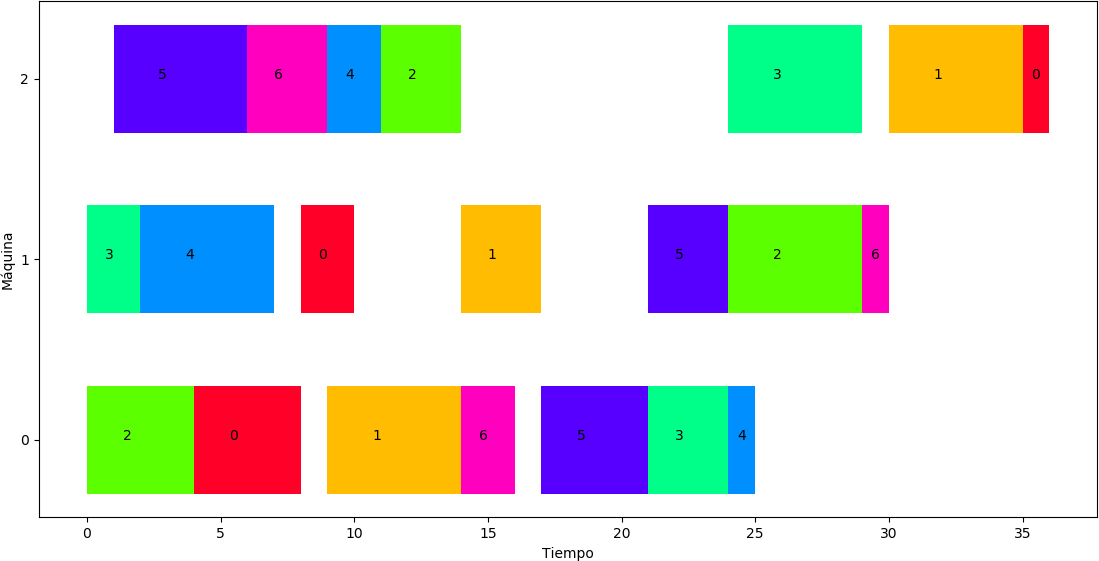
\includegraphics[scale = .45]{Imagenes/ganttfeas.png}
        \caption{Planificación factible pero no activa. Pueden observarse tiempos de inactividad que no se deben a ninguna restricción}
    \end{subfigure}
    \begin{subfigure}{.8\textwidth}
        \centering
        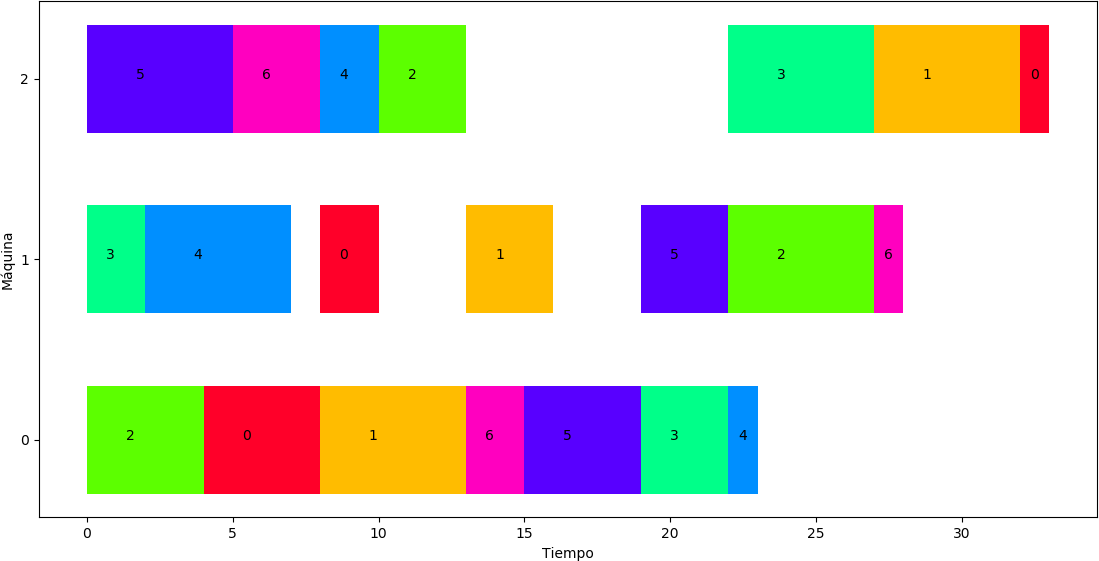
\includegraphics[scale = .45]{Imagenes/ganttsemi.png}
        \caption{Planificación semi-activa pero no activa. Solo hay tiempo de inactividad si se debe a las restricciones. Es posible reducir el tiempo de inicio de varias operaciones.}
    \end{subfigure}
    \begin{subfigure}{.8\textwidth}
        \centering
        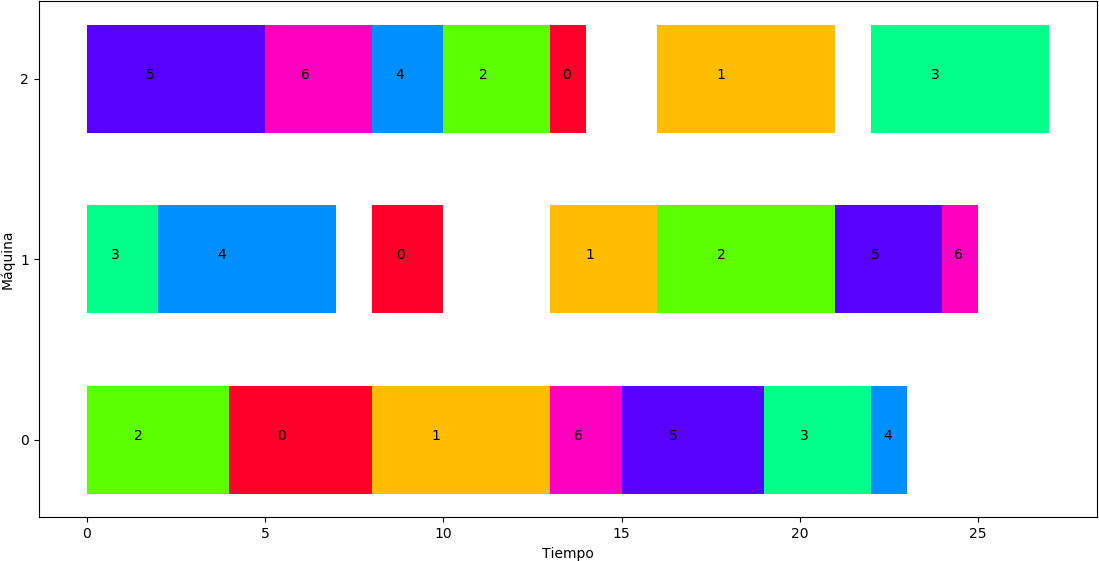
\includegraphics[scale = .45]{Imagenes/ganttactive.png}
        \caption{Planificación activa. No es posible reducir el tiempo de inicio de ninguna operación.} 
    \end{subfigure}
    \caption{Tres tipos de planificaciones para la instancia en \ref{tab:plantypes}}
        \label{fig:plantypes}
\end{figure}

%
Otra ventaja de centrarnos en las planificaciones semi-activas es que nos permite definir el concepto \textbf{ruta crítica}. 

%
Para una planificación semi-activa una \textbf{ruta crítica} es una secuencia ordenada de $k$ operaciones $(O_1,O_2,\dots,O_k)$ que cumple con las siguientes propiedades: el tiempo de inicio de la primera operación es cero y el de finalización de la última es igual al makespan de la planificación, el tiempo de inicio de la operación $i$ es igual al tiempo de finalización de la operación $i-1$ para $i>1$ y la operación $i-1$ es una dependencia de la operación $i$ para $i>1$.  

%
La ruta crítica se compone a su vez de una serie de \textbf{bloques críticos} que consisten en las secuencias de operaciones de la ruta crítica que se ejecutan de forma 
adyacente en la misma máquina. 
%
Es importante mencionar que una planificación semi-activa siempre tiene al menos una ruta crítica pero puede tener más de una a la vez.
%
Existen varias formas de determinar si una planificación es óptima, como se explicará más adelante, pero la más usada es el tiempo que toma terminar la última operación.
%
A este tiempo se le conoce como \textbf{makespan}. 
%
Sin pérdida de generalidad nos restringimos al caso en el que el tiempo requerido para procesar cada operación es un entero positivo.

% x Indicar que surgen dos tipos de dependencias, una en las propias máquinas (no puedes empezar antes que tu predecesora), y otra entre trabajos (no puedes empezar
% x hasta que acabe de predecesor del trabajo).
% x Es difícil definir el concepto de ruta crítica, sin decir que se hace uso de soluciones semi-activas, entonces creo que es importante definir aquí ese concepto
% x Hay que ser más formal al definir la ruta crítica, algo así como secuencia de operaciones tales que cada una tiene dependencia con la anterior, en la que la primera 
% x empieza en el tiempo 0 de planificación y la última termina en el tiempo makespan, y que cumple además que, cada operación empieza justo al terminar la operación anterior de la secuencia

%
El siguiente ejemplo sirve para mostrar los conceptos antes presentados en un caso práctico y simple.

\subsection*{Ejemplo}
Se muestra un ejemplo de una instancia con 3 máquinas y 2 trabajos en la tabla \ref{tab:inst}.
\begin{table}[H]
\centering
\begin{tabular}{@{}cccc@{}}
Trabajo & \multicolumn{3}{c}{\begin{tabular}[c]{@{}c@{}}Secuencia de procesamiento \\ (máquina, tiempo)\end{tabular}} \\ \midrule
0       & 0, 75                              & 2, 54                               & 1, 59                             \\ \midrule
1       & 0, 47                              & 2, 72                              & 1, 45   \\\hline                         
\end{tabular}
\caption{Instancia simple con 3 maquinas y 2 trabajos}
\label{tab:inst}
\end{table}

En la figura \ref{fig:gantt} se muestra una posible planificación para la instancia de ejemplo, visualizada mediante un diagrama de Gantt. En negro se marcan los trabajos que conforman la ruta crítica. 
\begin{figure}[H]
\centering
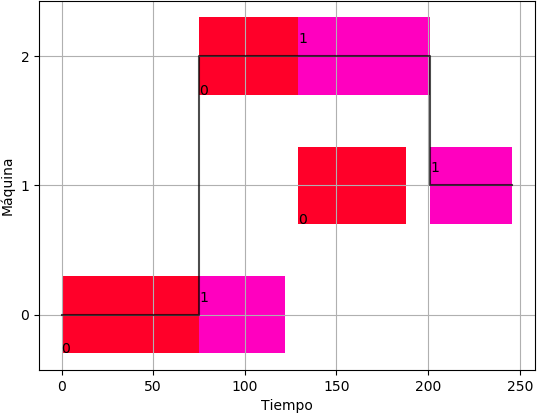
\includegraphics[scale=.7]{Imagenes/planejemplorc.png}
    \caption{Diagrama de Gantt de una planificación posible para la instancia mostrada en la tabla \ref{tab:inst}. Se marcan los trabajos que pertenecen a la ruta crítica con una línea}
\label{fig:gantt}
\end{figure}

Si bien es conveniente visualizar una planificación mediante un diagrama de Gantt como el mostrado anteriormente, resulta ventajoso representar computacionalmente 
estas planificaciones de otras formas. 
%
La representación de soluciones a un problema resulta ser una elección sumamente importante al momento de desarrollar, implementar y analizar los algoritmos que se 
propongan para resolver el problema~\cite{rothlauf2002representations}. 
%
En la siguiente sección se detallan dos formas de representación de especial importancia.

\subsection{Representación de planificaciones}
De manera general las representaciones para el JSP se pueden clasificar en\cite{Cheng1996}:
\begin{itemize}
    \item \textbf{Representación directa}: Se almacena el orden de los trabajos en cada máquina o sus tiempos de inicio y finalización.
    \item \textbf{Representación indirecta}: Se almacena información con la que se puede construir una planificación mediante un proceso de decodificación.
\end{itemize}

En este trabajo se utilizaron dos: una basada en permutaciones (representación directa) y las reglas de prioridad (representación indirecta).

\subsubsection*{Representación basada en permutaciones} 
En este modelo se identifica para cada máquina el conjunto de operaciones que deben procesarse en ella. Entonces una planificación se representa como un conjunto de $m$ permutaciones $(\sigma_0,\sigma_1,\dots,\sigma_m)$, donde $\sigma_i$ es la permutación de las operaciones que debe procesar la máquina $i$. Es decir que se asigna el orden de procesamiento de las operaciones cada máquina.
%
Esta representación no toma en cuenta el orden de procesamiento que deben cumplir las operaciones dentro de sus trabajos correspondientes por lo que no siempre representa planificaciones factibles.
%
Una forma de determinar si la permutación representa una planificación factible se construye un grafo dirigido $G=(V,A,E)$ en el que $V$ es un conjunto de nodos que representa las operaciones, las aristas $A$ representan la secuencia que deben seguir las operaciones dentro de un mismo trabajo y $E$ es otro conjunto de aristas que indica el orden de procesamiento en cada una de las máquinas. 

Pueden agregarse dos nodos de control que sirven como el nodo inicial o fuente del que dependen todas las operaciones ($S$) y final que depende de todos las operaciones ($*$), las restricciones de precedencia para las operaciones dentro de cada trabajo se representan como aristas dirigidas fijas llamadas aristas conjuntivas y las operaciones que deben procesarse en una misma máquina se unen mediante aristas llamadas disyuntivas cuya dirección se determina siguiendo la permutación dada. 
%
Para que una permutación represente una planificación factible su grafo asociado debe ser acíclico, puesto que la existencia de un ciclo en el grafo indica que hay una operación que está esperando a que se procese alguna otra operación que a su vez depende de que se procese la primera.
%
Una vez que se sabe que el grafo es acíclico se puede proceder a asignar tiempos de inicio y fin a cada operación asignando al nodo fuente ($S$) tiempo de inicio y finalización igual a cero y marcándolo como visitado. Posteriormente aplicando un algoritmo para recorrer el grafo cerciorándonos de solo visitar un nodo cuando ambas de sus dependencias han sido visitadas y asignarle un tiempo de inicio mayor que el mayor tiempo de finalización de sus dependencias y un tiempo de finalización igual al tiempo inicial más la duración de la misma.

Si se busca generar una planificación semi-activa, entonces el tiempo de inicio de la operación será el máximo de los tiempos de finalización de sus dependencias.

\subsubsection*{Ejemplo}
La planificación mostrada en la figura \ref{fig:gantt} tendría la siguiente representación como permutaciones:
\begin{align*}
\sigma_0 &= (O_{0,0}\,,\,O_{1,0})\\
\sigma_1 &= (O_{0,2}\,,\,O_{0,1})\\
\sigma_2 &= (O_{0,1}\,,\,O_{1,1})
\end{align*}
A partir de estas permutaciones se construye el grafo antes descrito y se escogen las direcciones de las aristas disyuntivas como se muestra en la figura \ref{fig:dgraph}. En este caso se verifica que el grafo es acíclico. 
\begin{figure}[h]
    \centering
    \begin{subfigure}{.8\textwidth}
        \centering
        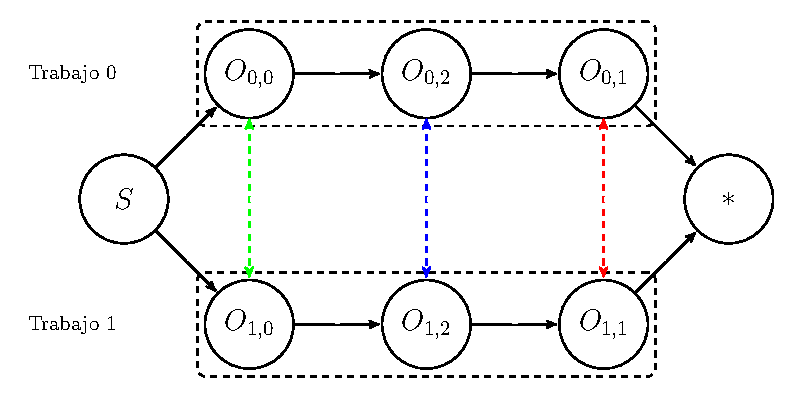
\includegraphics[width=.8\linewidth]{Imagenes/disyuntive.pdf}
        \caption{Representación de una instancia, los colores distinguen entre las tres máquinas.}
    \end{subfigure}
    \begin{subfigure}{.8\textwidth}
        \centering
        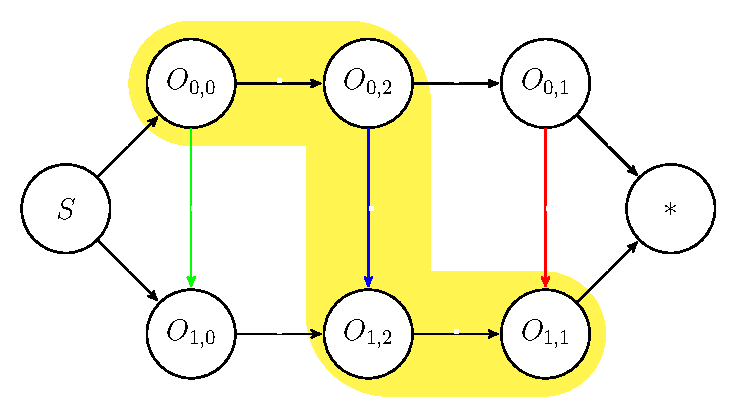
\includegraphics[width=.8\linewidth]{Imagenes/plandisyuntive.pdf}
        \caption{Planificación obtenida al fijar las aristas disyuntivas como en \ref{fig:gantt}. La ruta critica se resalta en amarillo}
    \end{subfigure}
\caption{Modelo de grafo disyuntivo para la instancia de ejemplo \ref{tab:inst}}
        \label{fig:dgraph}
\end{figure}

\subsubsection*{Representación basada en reglas de prioridad}
En esta representación una planificación se construye al aplicar un proceso de simulación en el que para cada maquina se construye una cola con las operaciones cuyas dependencias ya han sido procesadas. Inicialmente se tienen en las colas solo las operaciones iniciales de cada trabajo. Una vez que se tiene esto se utiliza una regla de prioridad para elegir qué operación debe planificarse en qué máquina. Se actualizan las colas para las máquinas que lo requieran y se continua con este proceso hasta completar la planificación (vaciar las colas).

Existen muchas reglas de prioridad que toman en cuenta cosas como la duración de la operación, la cantidad de operaciones restantes, la duración del trabajo al que pertenece una operación, entre muchas otras. La calidad de la planificación construida depende de la regla de prioridad que se utilice y de la estructura de la instancia en sí.

